\documentclass[aspectratio=169]{beamer}
\usepackage{graphicx,tikz,pgfpages}
\setbeamertemplate{navigation symbols}{}
\ifdefined\presenternotes\setbeameroption{show notes on second screen=right}\else\setbeameroption{hide notes}\fi
\begin{document}
\begin{frame}[plain]
\begin{tikzpicture}[remember picture,overlay]\node at (current page.center) {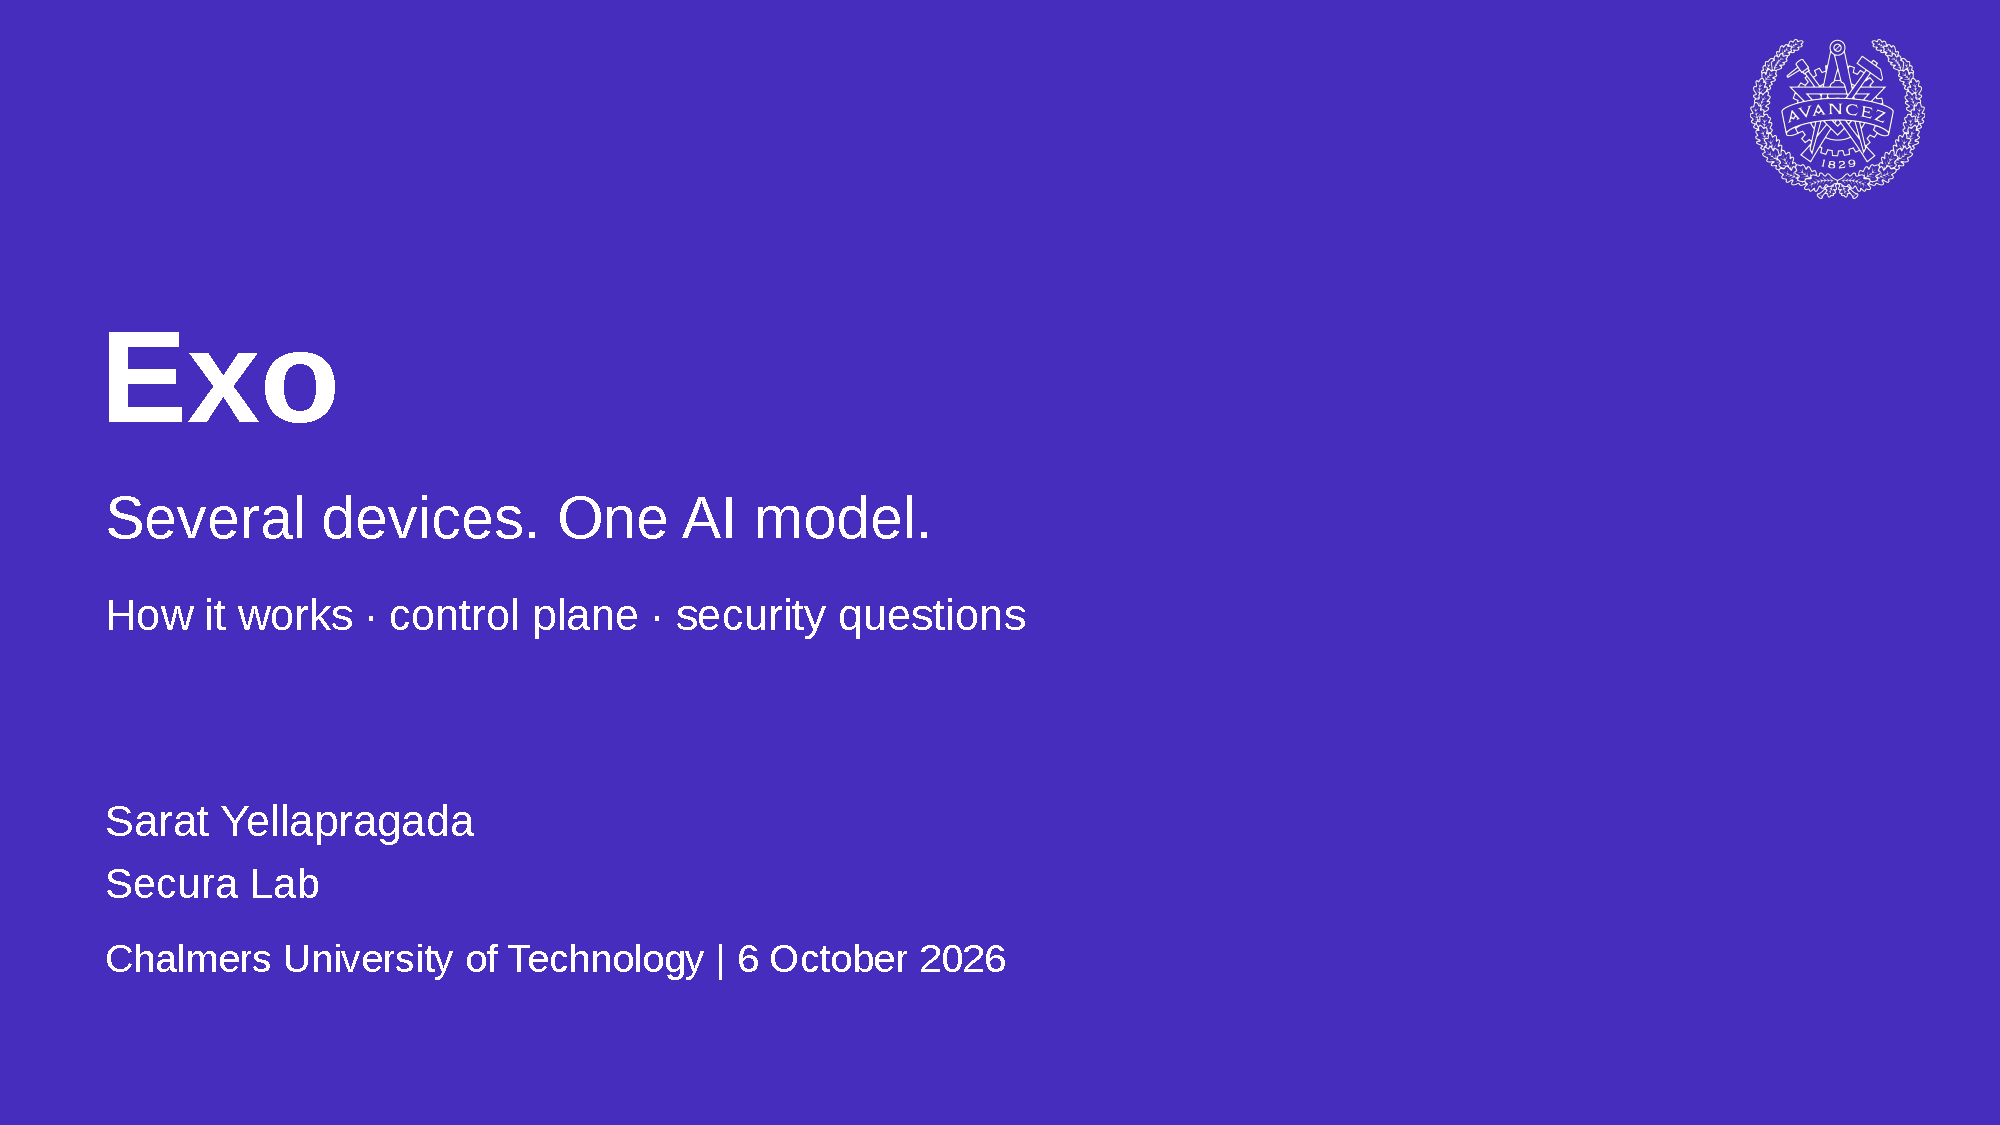
\includegraphics[width=\paperwidth,height=\paperheight]{slides/01.pdf}};\end{tikzpicture}
\note{Exo connects devices into a local AI inference cluster. A large model can be divided among devices rather than requiring its entire memory footprint on one device. This talk answers four questions: what problem Exo solves, how its architecture works, where the control plane sits, and which security problems are worth investigating. The architecture is source-reviewed at commit 21a54c5ea0230a3bec1e1a786d200126c7e34ec6; our measurements are one private, model-free local trial per experiment arm. We do not present inference benchmarks or a public-swarm result.

Sources: pinned Exo README, local audit report.}
\end{frame}
\begin{frame}[plain]
\begin{tikzpicture}[remember picture,overlay]\node at (current page.center) {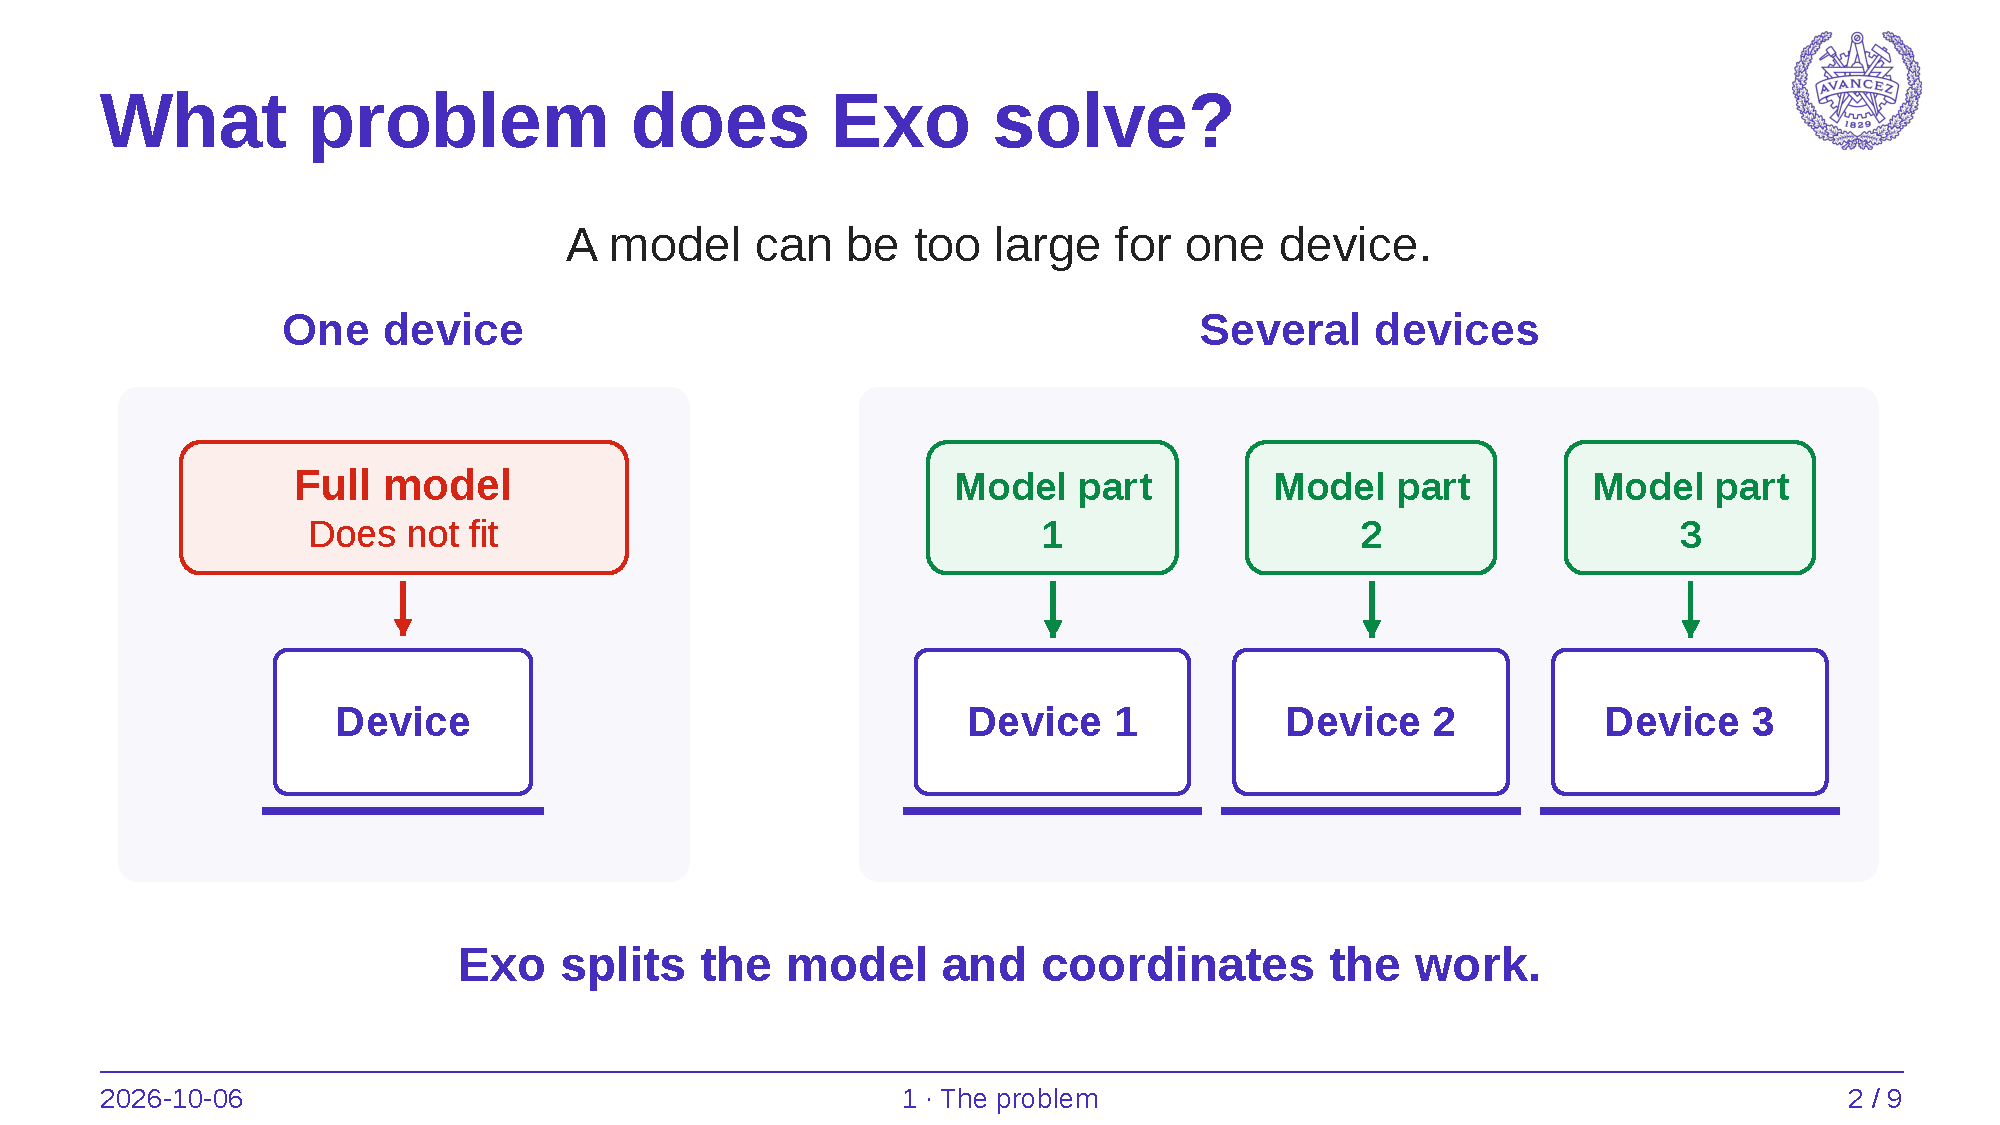
\includegraphics[width=\paperwidth,height=\paperheight]{slides/02.pdf}};\end{tikzpicture}
\note{The main problem is model capacity. Model weights plus runtime state may exceed one device's available memory. Exo can place parts of a model on multiple compatible devices so that they jointly execute inference. The drawing is illustrative: it does not assert a particular RAM requirement, equal-sized partitions, or a speedup. The actual partition depends on model constraints, available memory, supported backends, and usable network links. Exo supports pipeline and tensor parallel arrangements; the picture simply shows that devices share the model's work. Adding devices also adds communication, so faster inference is not guaranteed by this capacity argument.

Sources: purpose and features, placement constraints.}
\end{frame}
\begin{frame}[plain]
\begin{tikzpicture}[remember picture,overlay]\node at (current page.center) {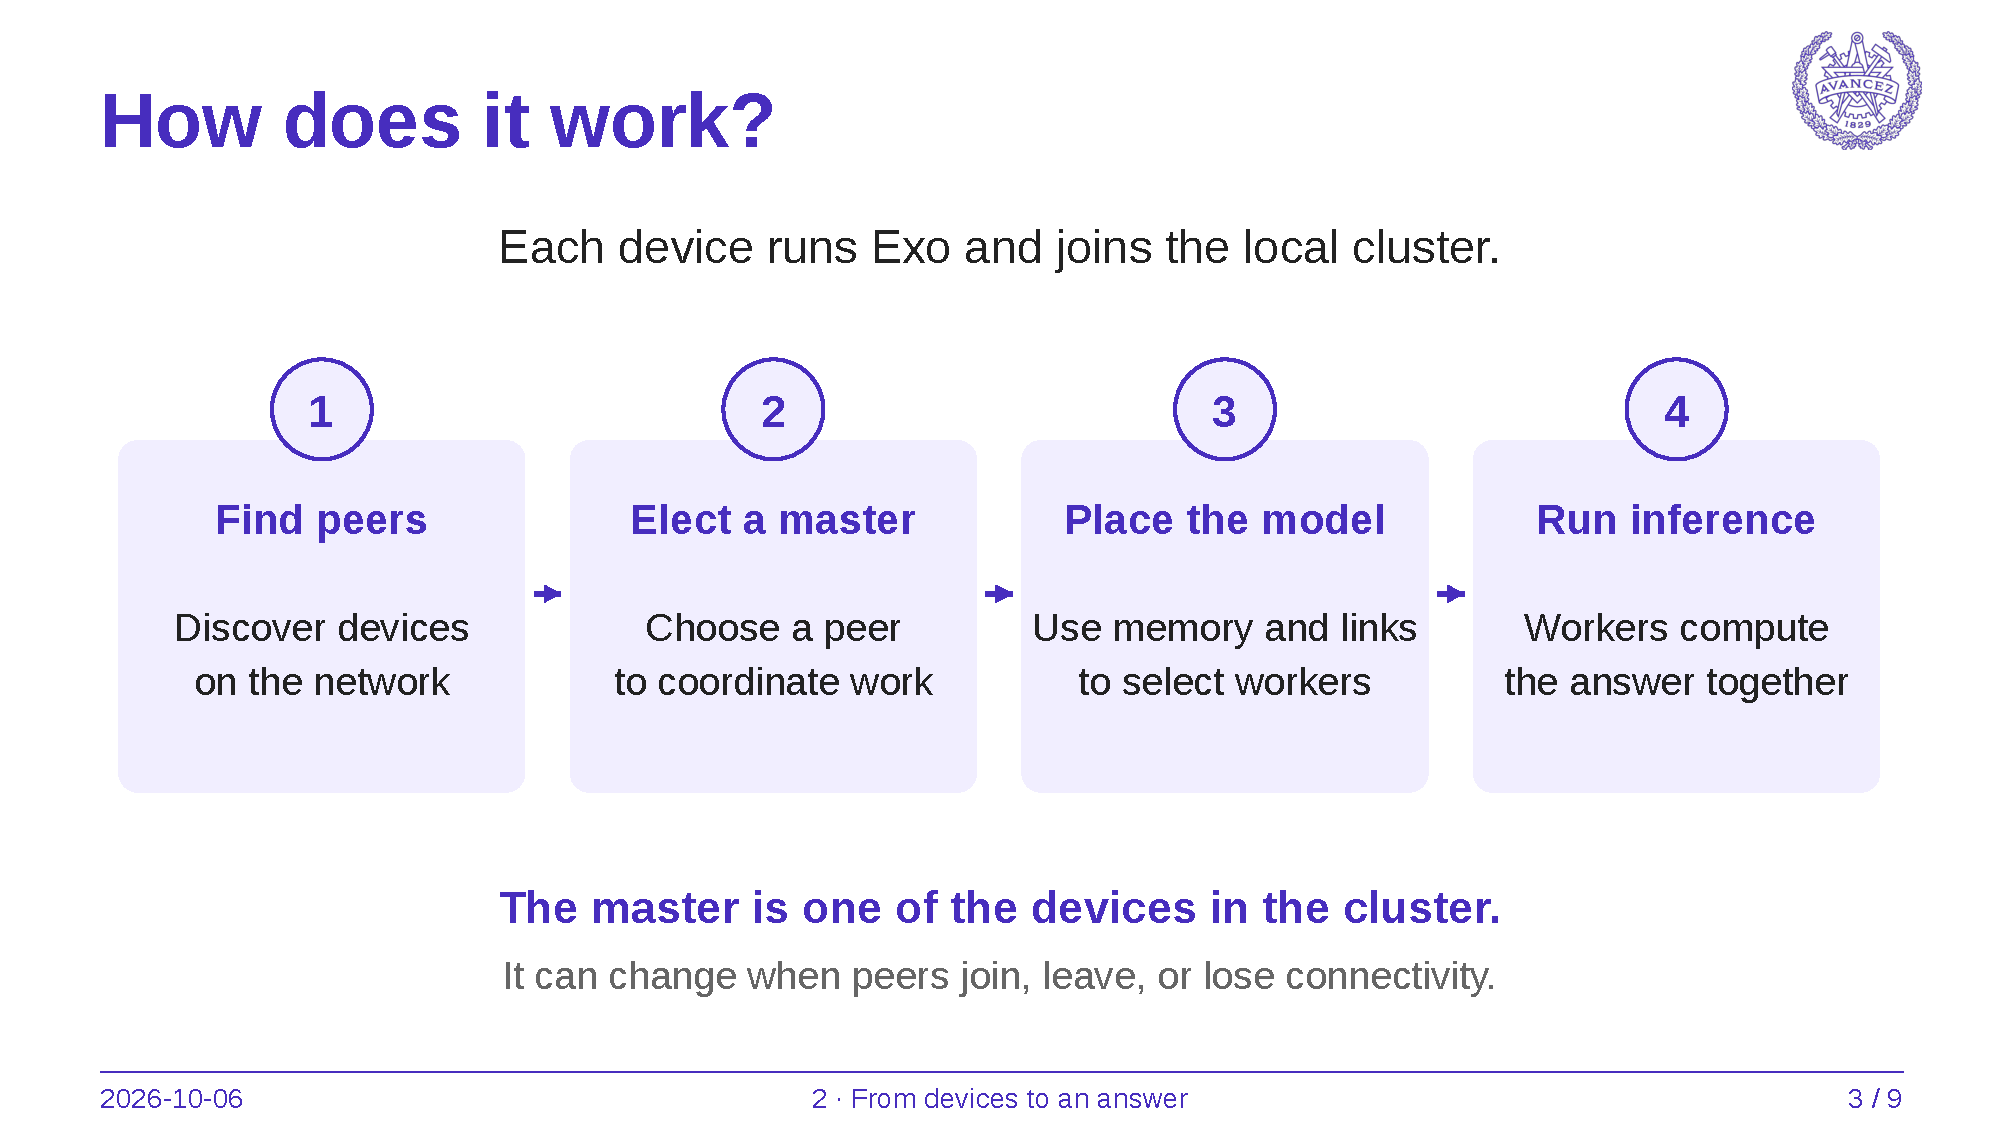
\includegraphics[width=\paperwidth,height=\paperheight]{slides/03.pdf}};\end{tikzpicture}
\note{Devices discover namespace-compatible peers using IPv6 multicast, then establish Zenoh connections. Election selects a coordinator, called the Master in the source. Each normal worker reports information such as available RAM, network interfaces, and supported backends. The master uses device profiles and a separately constructed placement topology to choose a model instance's workers and assign shards. That topology includes usable socket or RDMA links; it is not merely the list of discovered peers. Selected workers load their assignments. For an inference request, an API issues a command, the master creates tasks for a suitable model instance, and the assigned workers execute them and return output through the event stream. Discovery and elections also happen as connectivity changes; this is a high-level lifecycle, not a new election for every prompt. A connection change can trigger an election without changing the final master. Recovery behavior after failures still needs testing.

Sources: discovery, election, device reports, placement, request scheduling.}
\end{frame}
\begin{frame}[plain]
\begin{tikzpicture}[remember picture,overlay]\node at (current page.center) {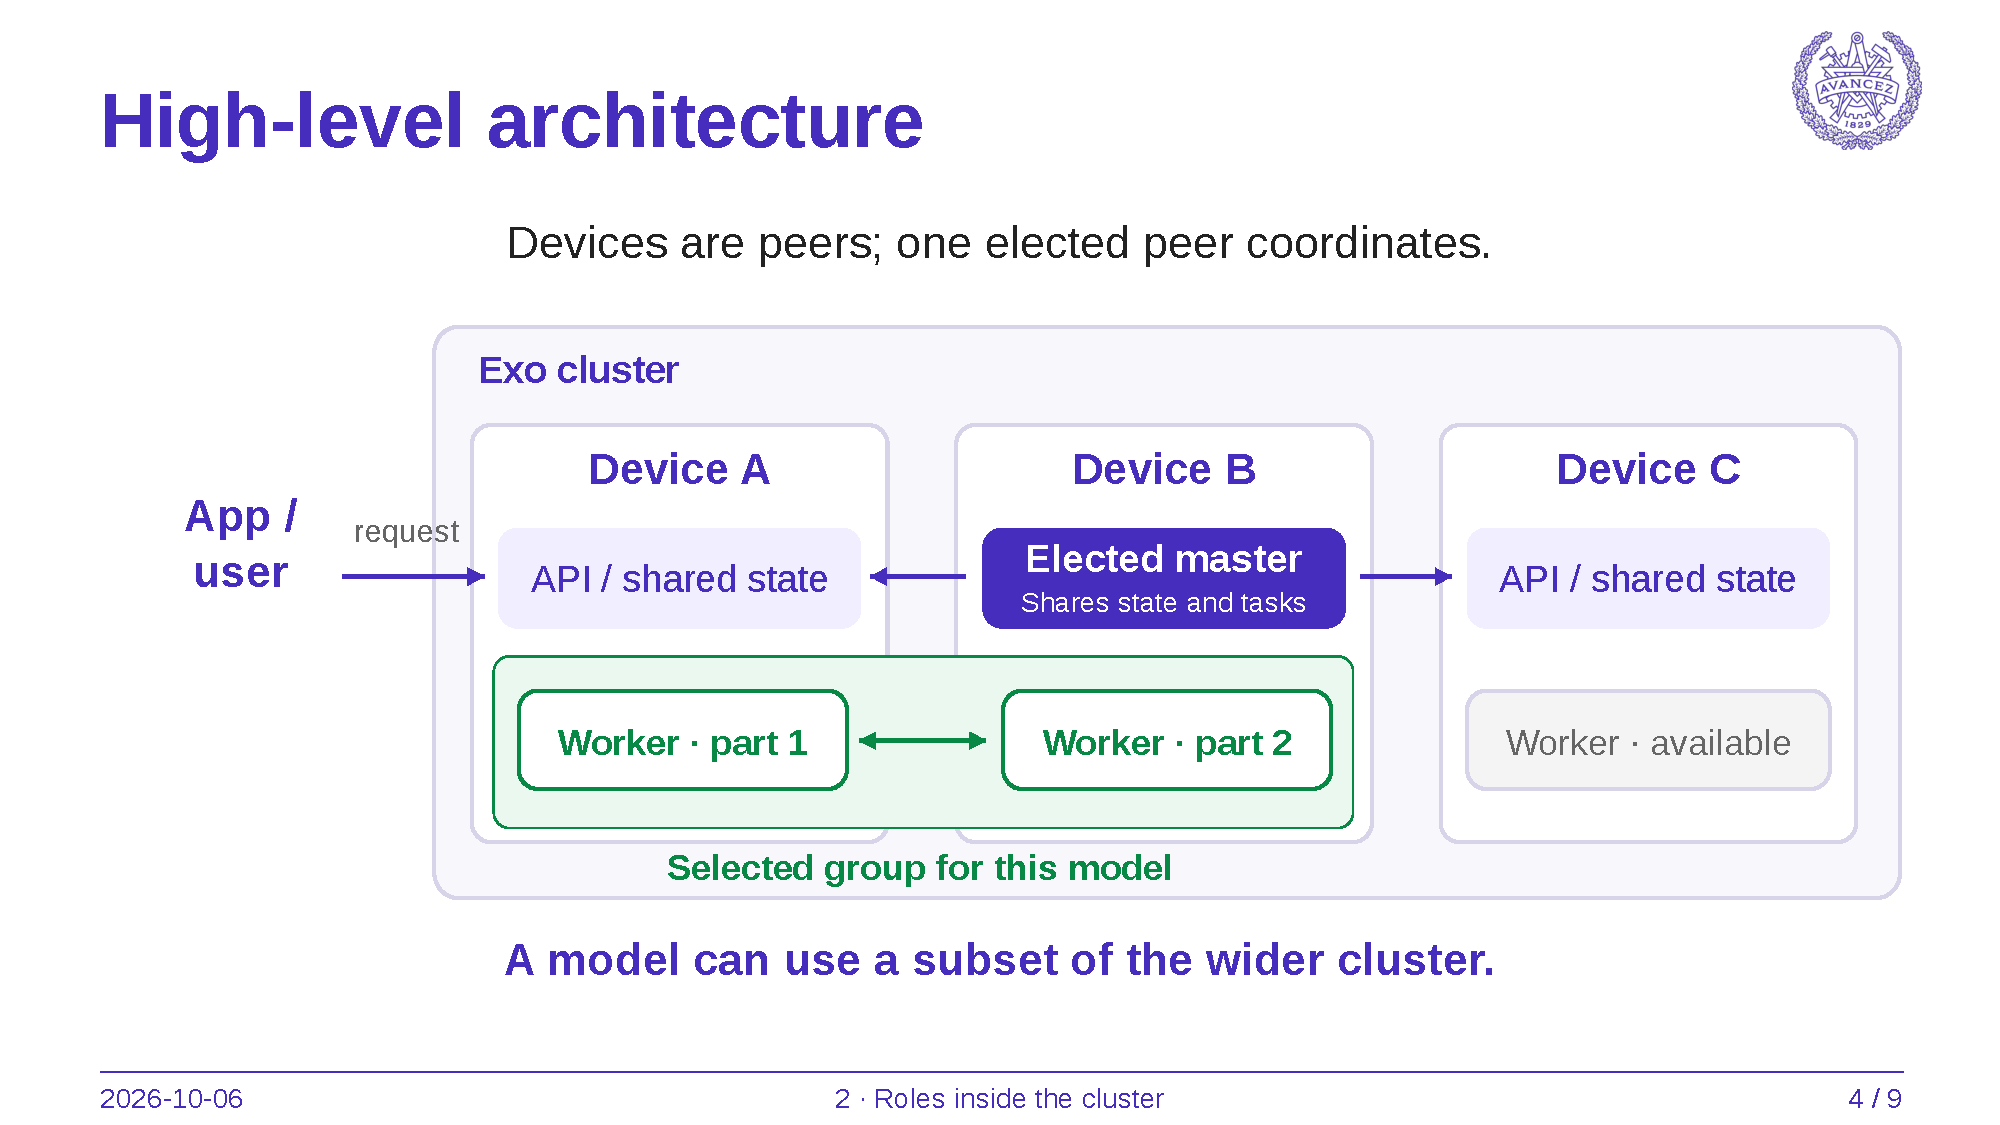
\includegraphics[width=\paperwidth,height=\paperheight]{slides/04.pdf}};\end{tikzpicture}
\note{This is a diagram of logical roles inside three physical devices. The API can run on any device; the app enters through A's API in this example. Every normal node has an API and worker unless disabled. B is the elected master and may also execute inference as a worker. All nodes initially create a Master object, but election results determine which one is active. The active master indexes events and coordinates placement and tasks. A and B are selected for this model; C is discovered but its worker is not selected for this instance. Instance assignments therefore form a group within the wider cluster, unlike Hivemind's temporary gradient-averaging groups. An Exo model instance's group exists to execute its model. The shaded group is not a separate discovery network. The figure omits B's own API and replicated-state box for space. The master is hosted by a peer, rather than drawn as a permanent external service. The purple arrows show the master distributing shared state and tasks; API commands travel back through peer messaging, which is omitted to keep the drawing simple. This is not a picture of physical network hops or the full peer connection graph. The green link summarizes worker communication without specifying a particular parallelism mode.

Sources: node components, promotion and demotion, instance assignments, per-instance topology.}
\end{frame}
\begin{frame}[plain]
\begin{tikzpicture}[remember picture,overlay]\node at (current page.center) {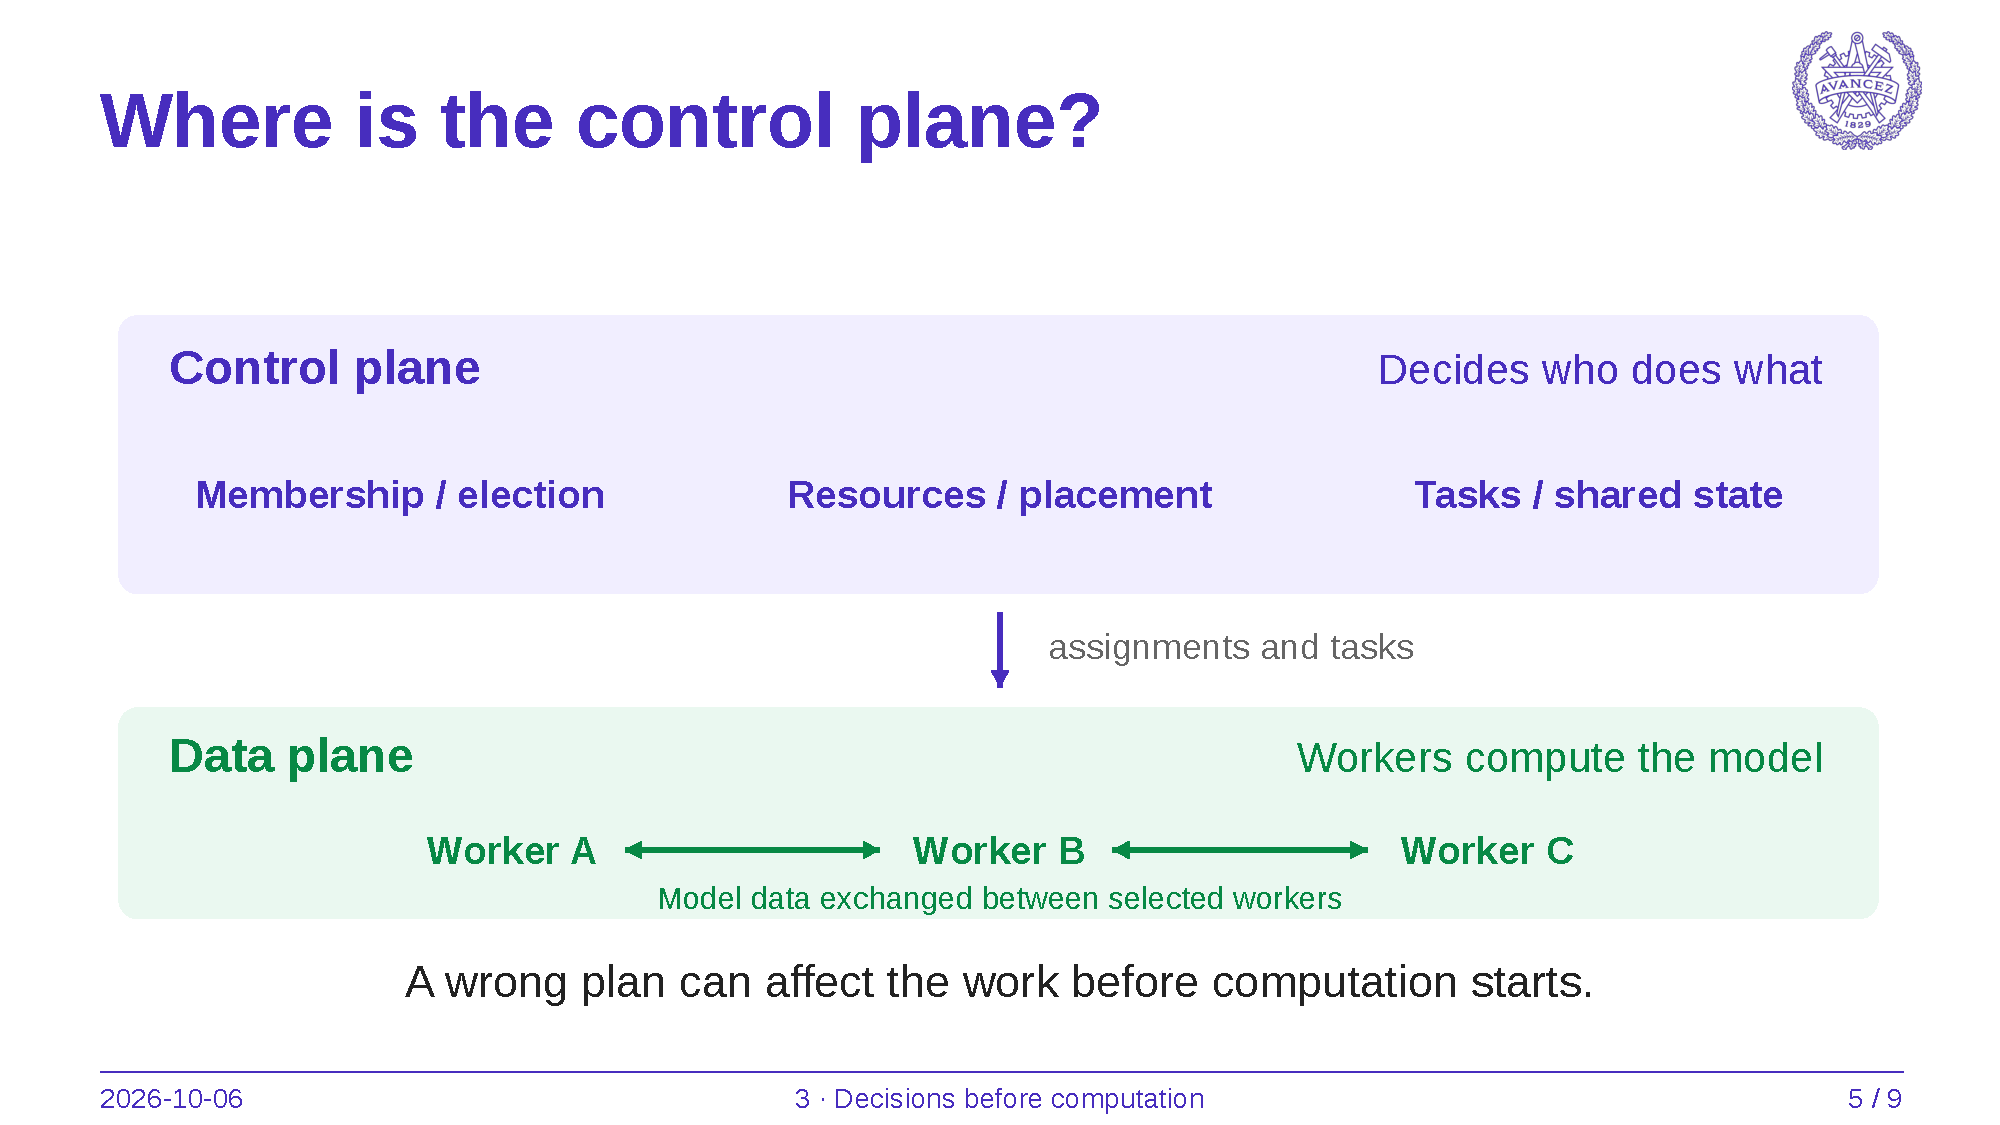
\includegraphics[width=\paperwidth,height=\paperheight]{slides/05.pdf}};\end{tikzpicture}
\note{The control plane is the part that decides who belongs to the cluster, which peer is master, which device information to trust, where to place a model, and which tasks should run. The master broadcasts indexed events so peers maintain a common view. Model execution is the work those decisions direct: workers use their model shards and exchange model-parallel data. This separation is by function, not by packet size or a perfectly separate transport. Zenoh pub/sub carries election messages, commands, state events, and also inference task payloads and generated output chunks. MLX distributed carries communication between model workers, including tensor send/receive and gather operations. For security research we can initially test decisions and state with synthetic metadata, without loading a large model. A false accepted advertisement may lead to a wrong plan, but we must test that next step rather than assume it.

Sources: typed topics, Zenoh messaging, master indexing, MLX group initialization, model-parallel communication.}
\end{frame}
\begin{frame}[plain]
\begin{tikzpicture}[remember picture,overlay]\node at (current page.center) {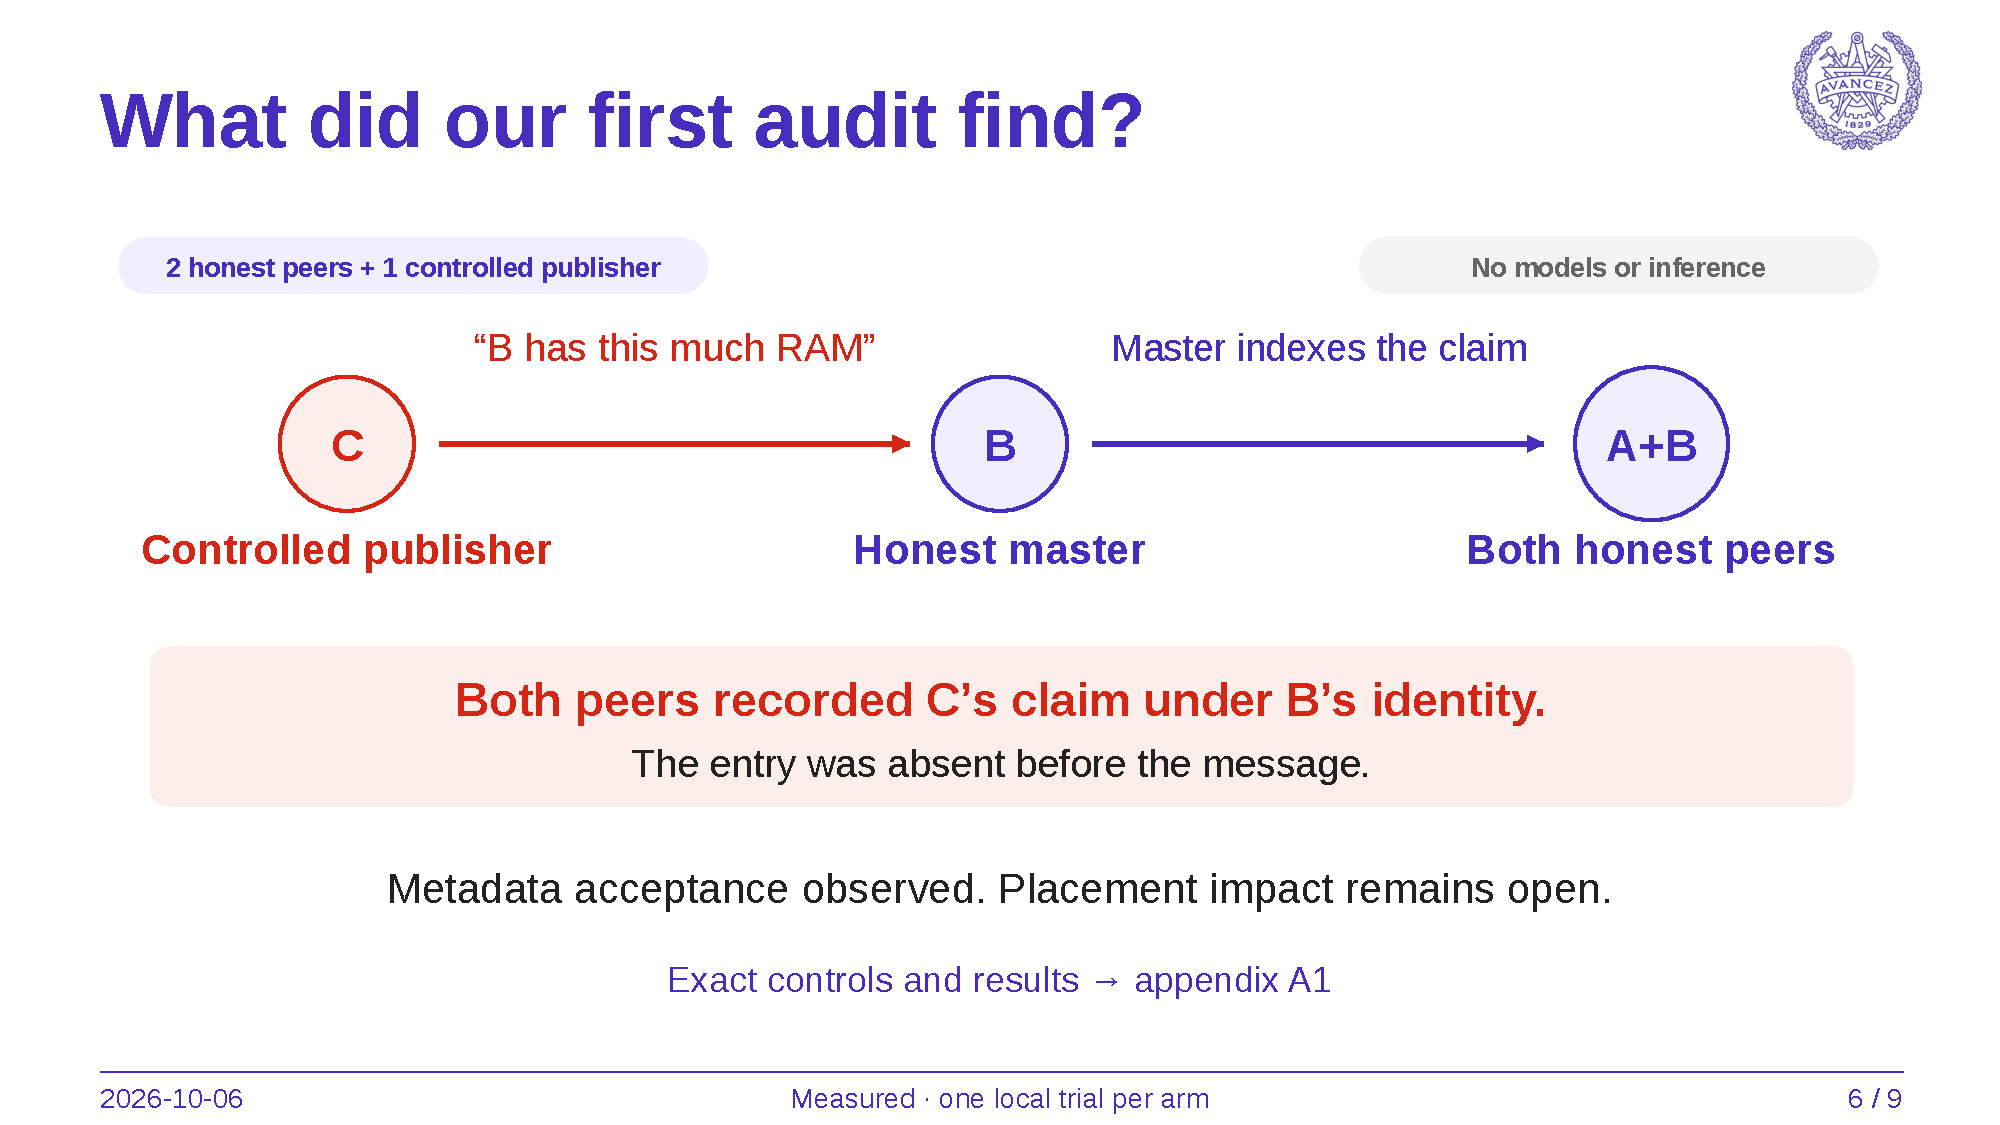
\includegraphics[width=\paperwidth,height=\paperheight]{slides/06.pdf}};\end{tikzpicture}
\note{The local experiment used two honest, unmodified Exo coordinator processes and a controlled publisher using the real Router. C had no master, worker, API, or election role. After A and B had converged and C's transport was connected, C sent one resource event whose claimed node ID was B's, although C's transport ID was distinct. The synthetic available RAM value was exactly 136,164,352 bytes. B happened to be the elected master in this arm. It indexed the event, emitted a matching global event with the current master origin/session, and both honest API snapshots then showed the value under B's ID. The entry was absent in both before snapshots. Peer identities and sessions stayed unchanged. The self-advertisement positive control also worked, and the no-send baseline produced no entry. This is measured acceptance of a claim about another node, not proof that a real worker's report was overwritten or that inference was affected: workers were disabled. We also have not established that this behavior crosses the project's intended authorization boundary. The finding is a concrete lead for further control-plane research.

Evidence: report, probe envelopes, before, after, control.}
\end{frame}
\begin{frame}[plain]
\begin{tikzpicture}[remember picture,overlay]\node at (current page.center) {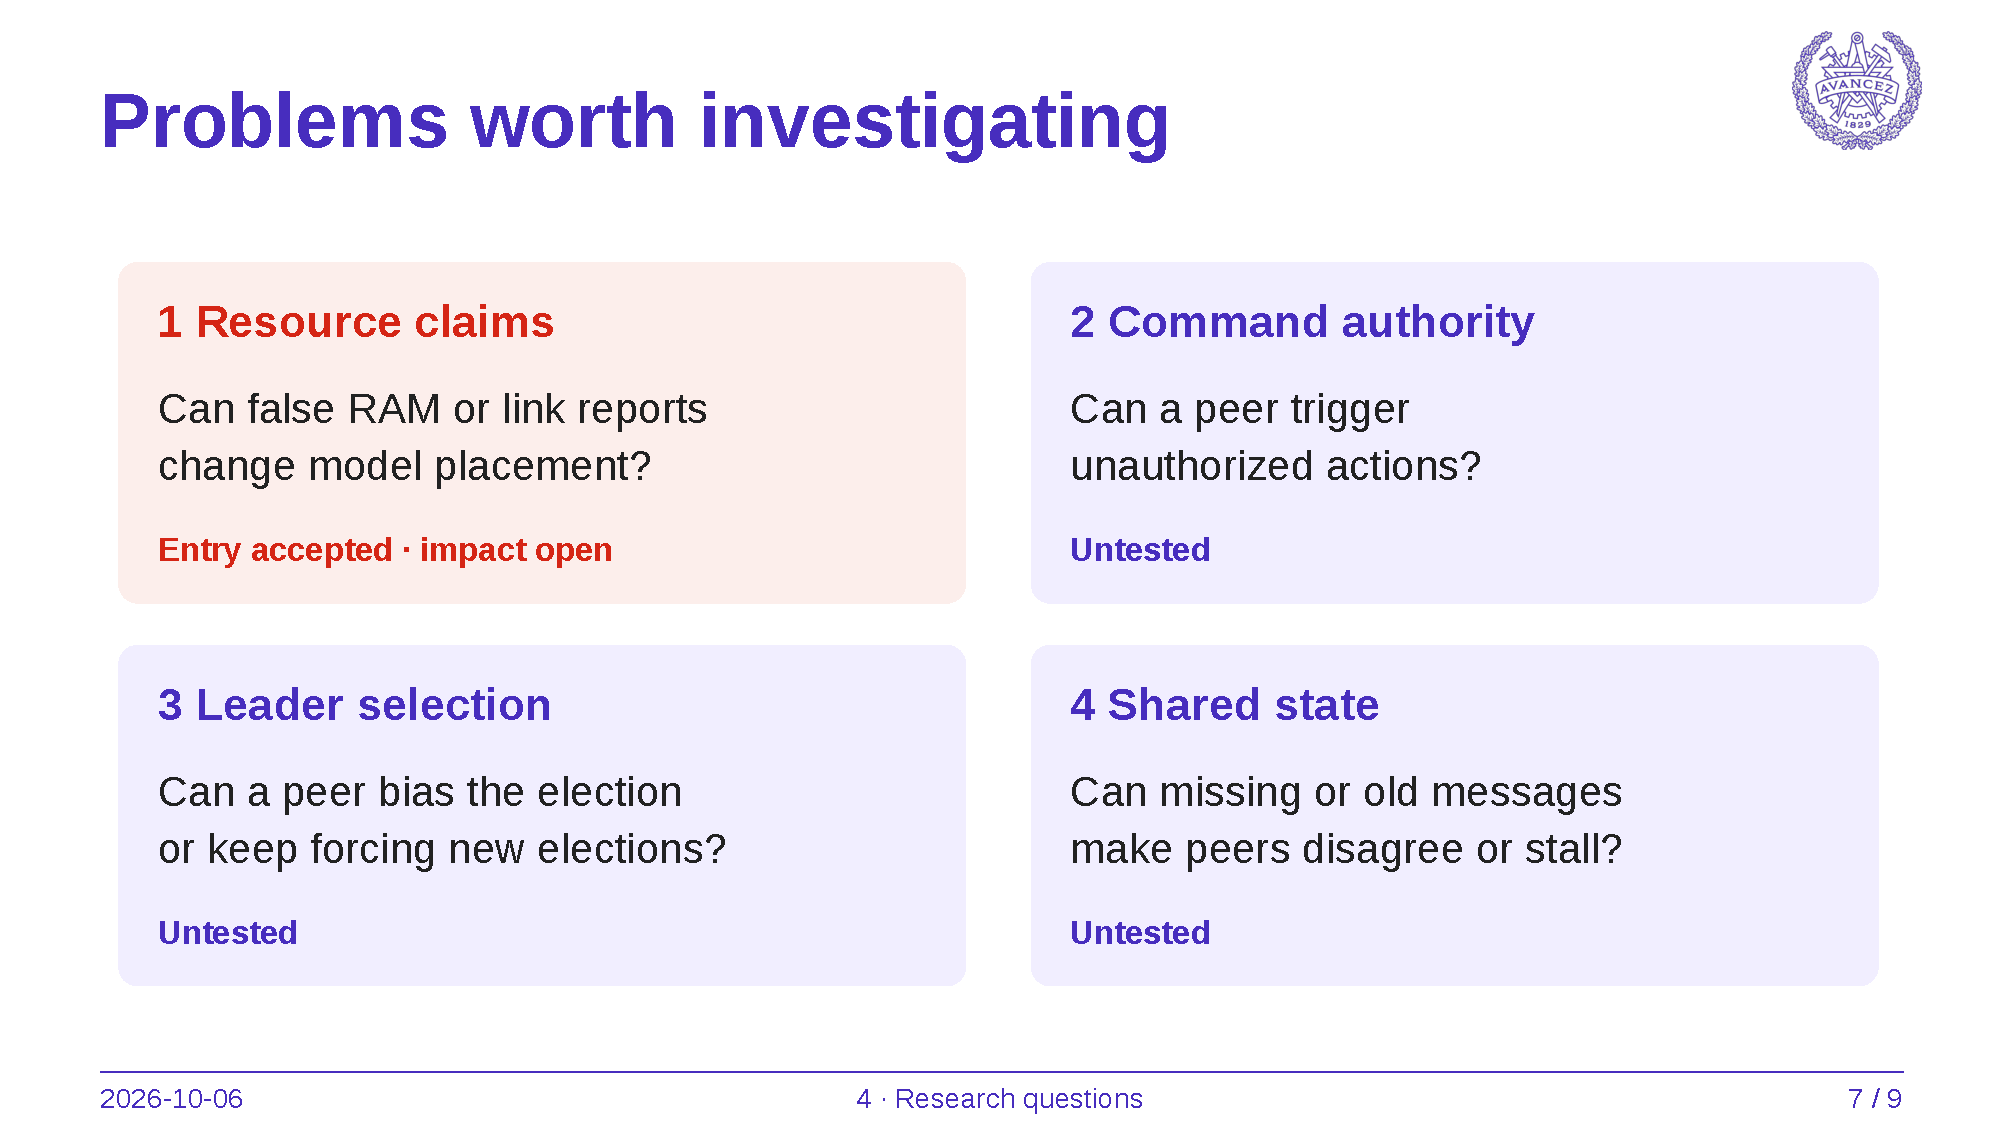
\includegraphics[width=\paperwidth,height=\paperheight]{slides/07.pdf}};\end{tikzpicture}
\note{These are research questions, not four validated vulnerabilities. Our first priority is to connect the measured resource-claim acceptance to a consequential decision. Use an honest baseline, fake model metadata, and a controlled changed RAM or network profile; then compare selected nodes and assignments. This can test placement without downloading weights. We still need to test competition with normal worker reports and the trust boundary.

Command authority asks which peers or clients may create, cancel, or delete work and whether those actions are bound to an authorized origin. Inspect both API admission and network command/event handling; a local open API's existence alone is not a vulnerability. Leader selection asks whether self-reported election fields, especially clock, seniority, and commands seen, can bias leadership or cause repeated elections. This requires an attacker able to reach the same cluster's messaging path; it is not an Internet-wide takeover claim. Shared state asks what happens under gaps, conflicting ordering, stale sessions, partitions, restart, and rejoin. Our exact duplicate test indexed once; the constructed session mismatch was not observed. Those controls do not establish safety for other sequences or recovery conditions. All active tests should remain in the private lab until a public operator and scope are agreed.

Sources: placement, commands, master command handling, election fields, replicated event handling, ordered buffer.}
\end{frame}
\begin{frame}[plain]
\begin{tikzpicture}[remember picture,overlay]\node at (current page.center) {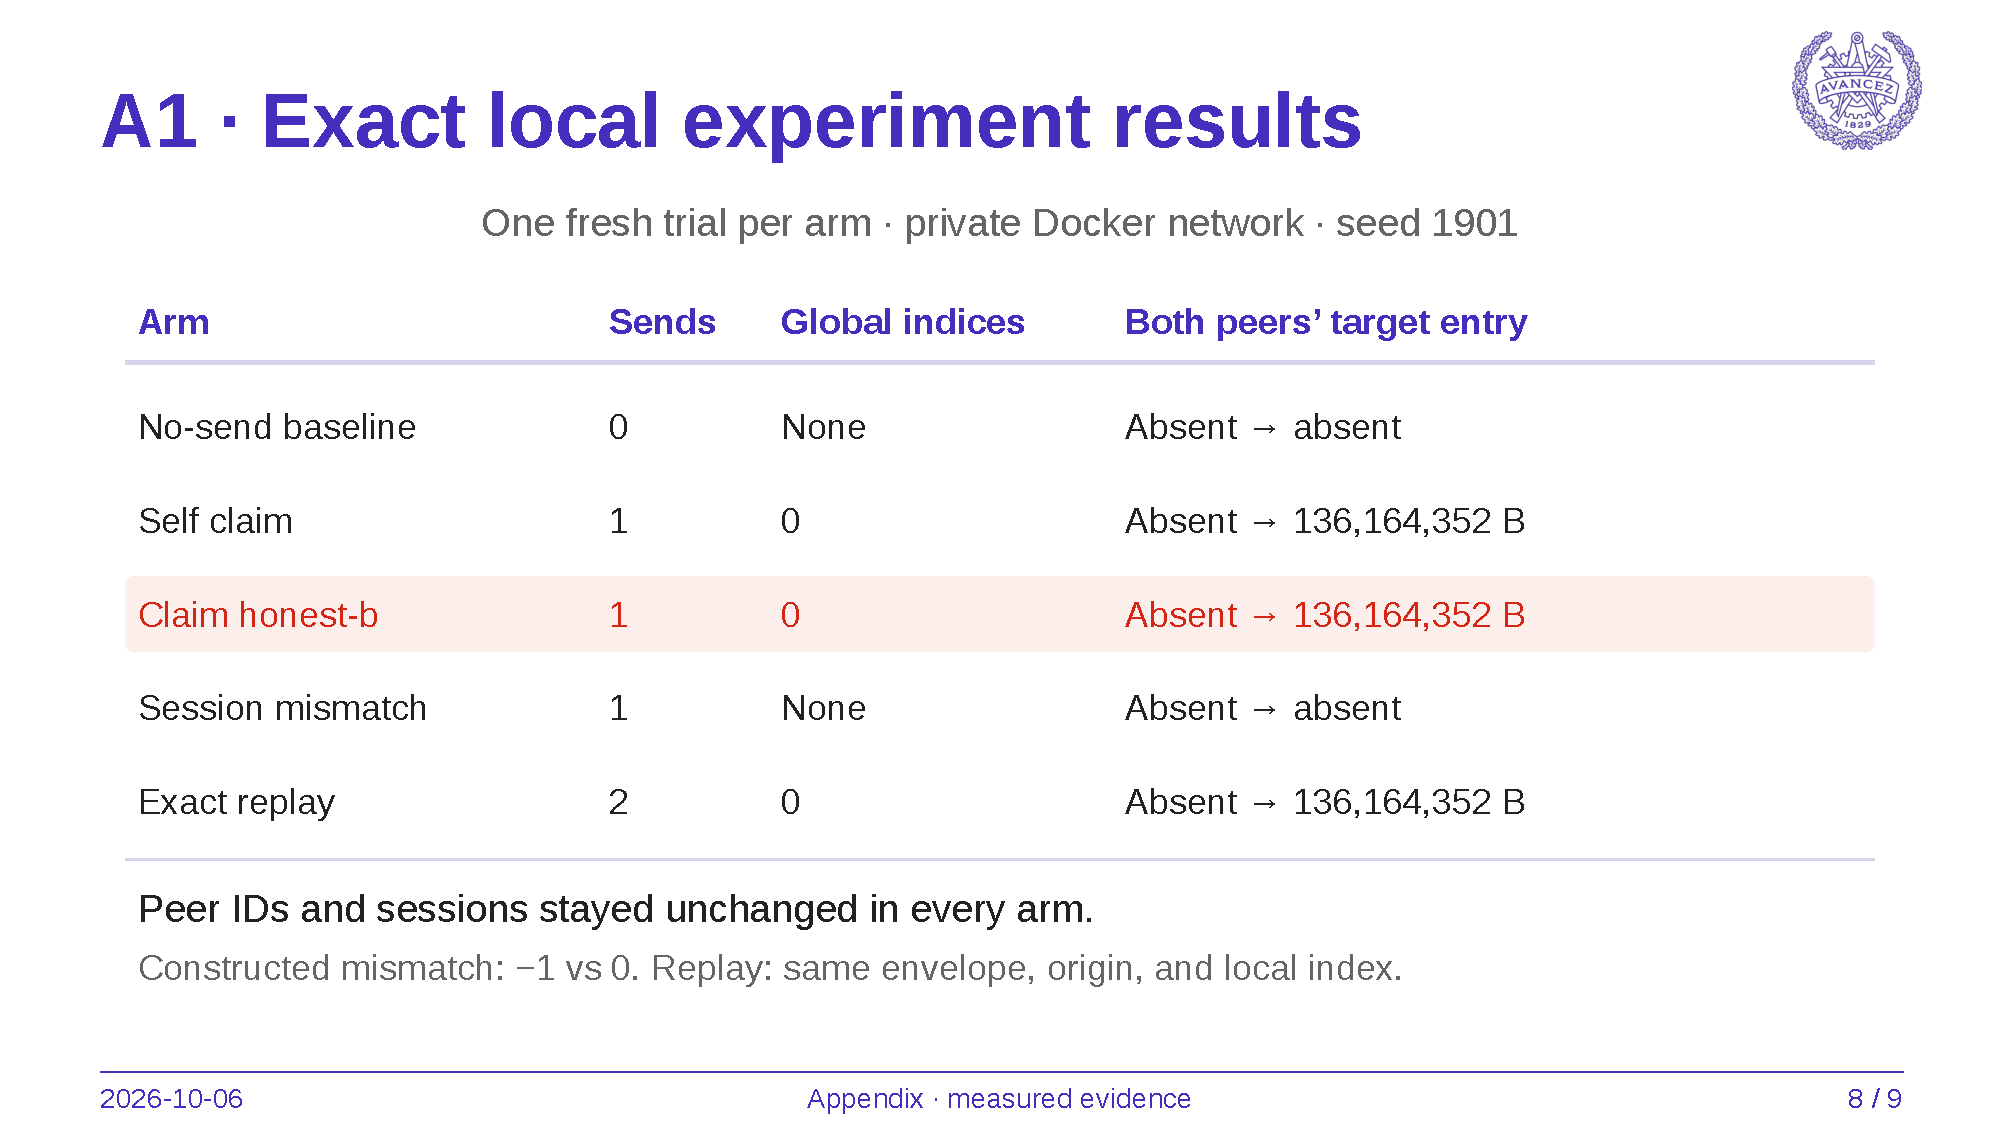
\includegraphics[width=\paperwidth,height=\paperheight]{slides/08.pdf}};\end{tikzpicture}
\note{Each row is one fresh private arm, with two honest peers and the same third-transport role, not a deployment success rate. The no-send arm had zero publications. The self and forged arms each had one publication and one distinct observed global index. Both targets were absent before and held 136,164,352 available bytes afterward. In the forged arm the target was honest-b, which was also the master. The mismatch arm used a constructed clock of -1 while the current session clock was 0; no matching global event or target entry was observed during its bounded window. This was not a message captured from a previously active session, and there was no explicit rejection response. The replay arm recorded two byte-identical local publications, sent the second after the first indexed acknowledgement, and observed one global index. The master trace contained one matching indexing line. It did not exercise a fresh origin or a fresh local index. Separate code inspection shows that the master filters session mismatches and the ordered buffer drops an already-consumed local index. Those explanations are source inferences alongside these measurements. No models were loaded. Helper checks passed, all outcomes reproduced from saved raw records, and run containers/networks were removed while evidence and state volumes were retained.

Evidence: summary, manifest and lab copies, raw outcome verification, resource captures, cleanup. Each arm directory retains probe.jsonl, before/after snapshots, consensus records, peer logs, and command records.}
\end{frame}
\begin{frame}[plain]
\begin{tikzpicture}[remember picture,overlay]\node at (current page.center) {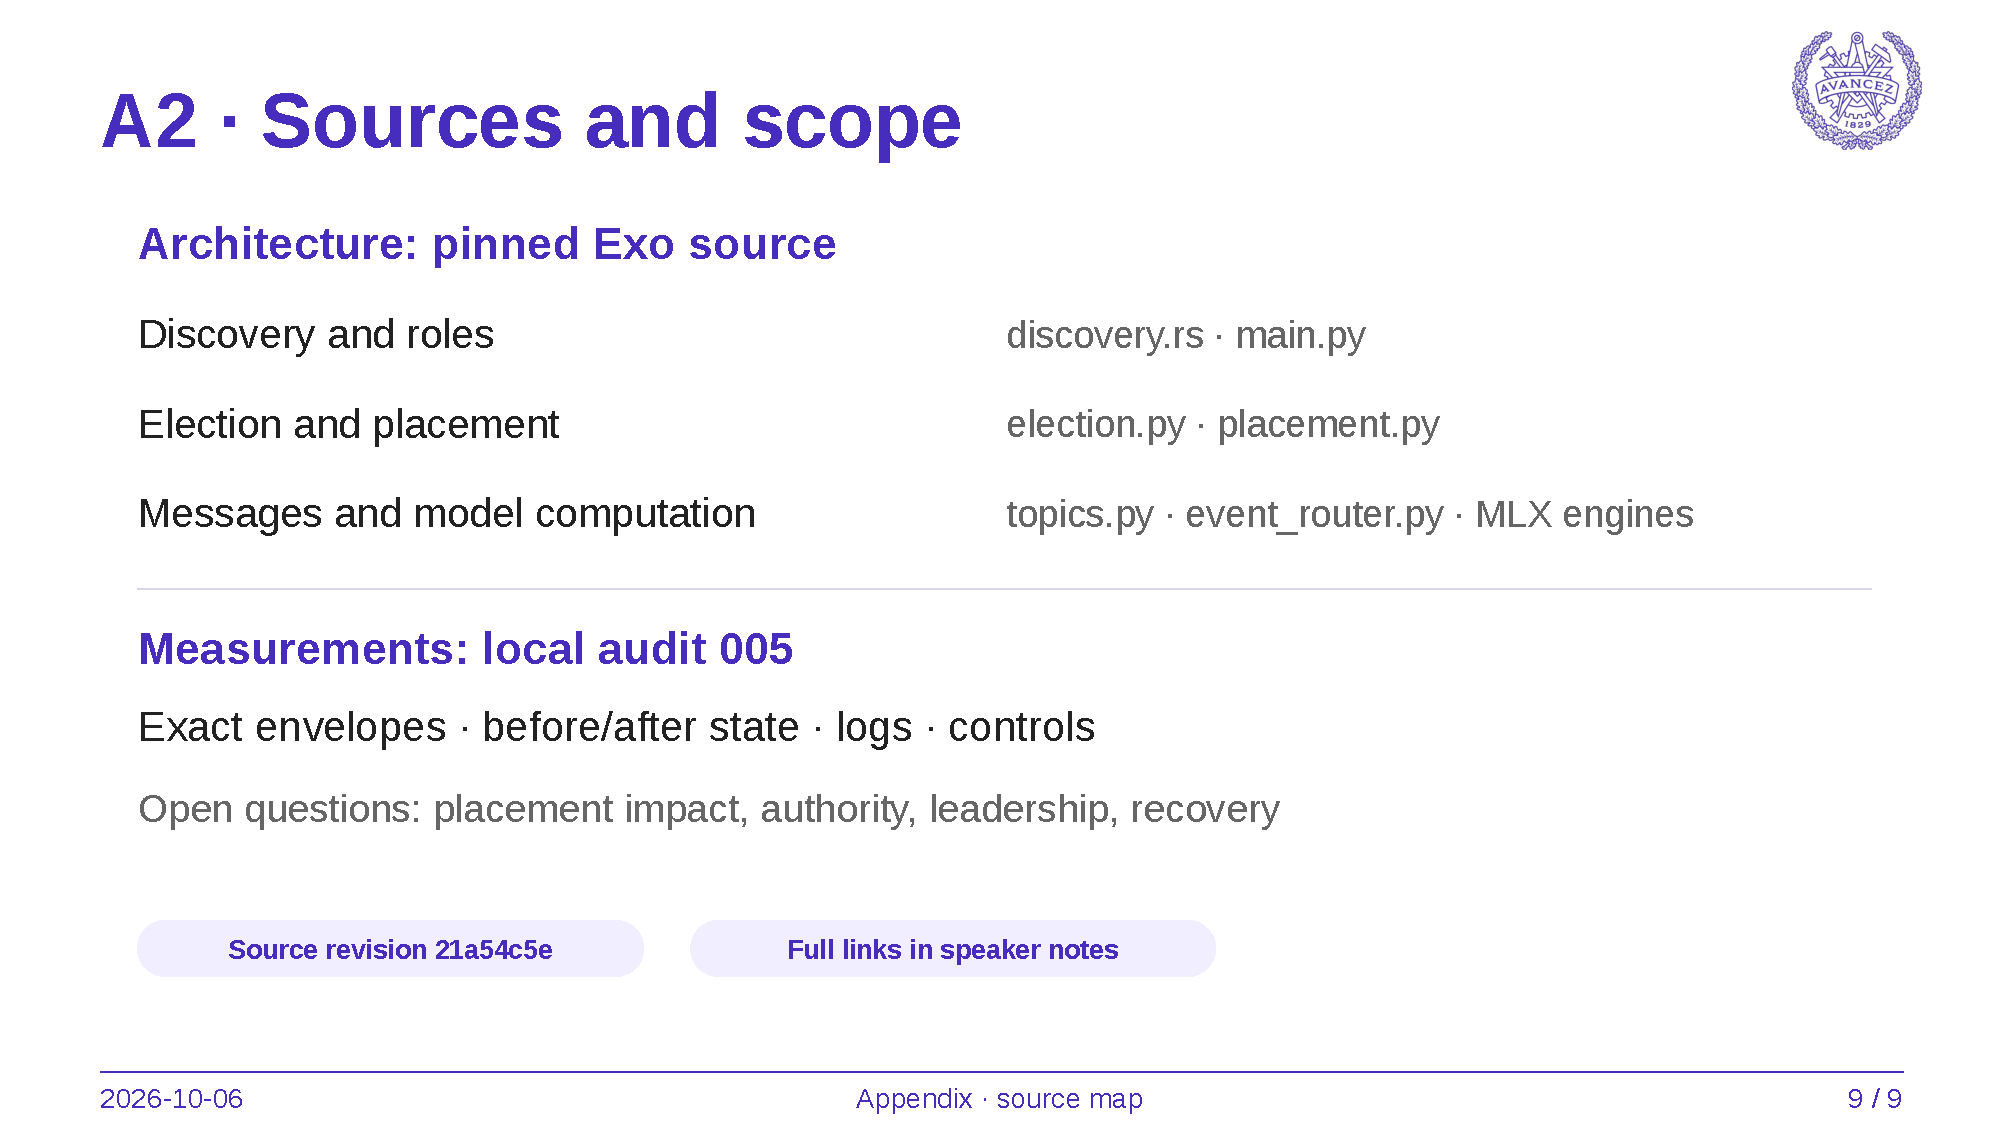
\includegraphics[width=\paperwidth,height=\paperheight]{slides/09.pdf}};\end{tikzpicture}
\note{The deck describes the reviewed Exo implementation, not a claim about every future version or deployment. The source pin is 21a54c5ea0230a3bec1e1a786d200126c7e34ec6. All primary source links below use that full commit. The observed result comes from the preserved 2026-10-06 local audit; no public swarm or WAN experiment was run. Proposed consequences and new attacks remain open questions.

Primary sources:

- Exo purpose
- Node roles
- IPv6 discovery
- Zenoh transport
- Election
- Worker reports
- Placement
- Master processing
- Shared event handling
- MLX communication
- Local report and evidence}
\end{frame}
\end{document}
